\documentclass[10pt]{report}
\usepackage{/Users/bradenhoagland/latex/math}

\lhead{Braden Hoagland}
\chead{HW 4}
\rhead{}

\renewcommand{\theenumi}{\alph{enumi}}

\begin{document}
%\tableofcontents

\begin{exer}[]
\S 4.1: \#1.
\end{exer}
\begin{figure}[H]
	\centering
	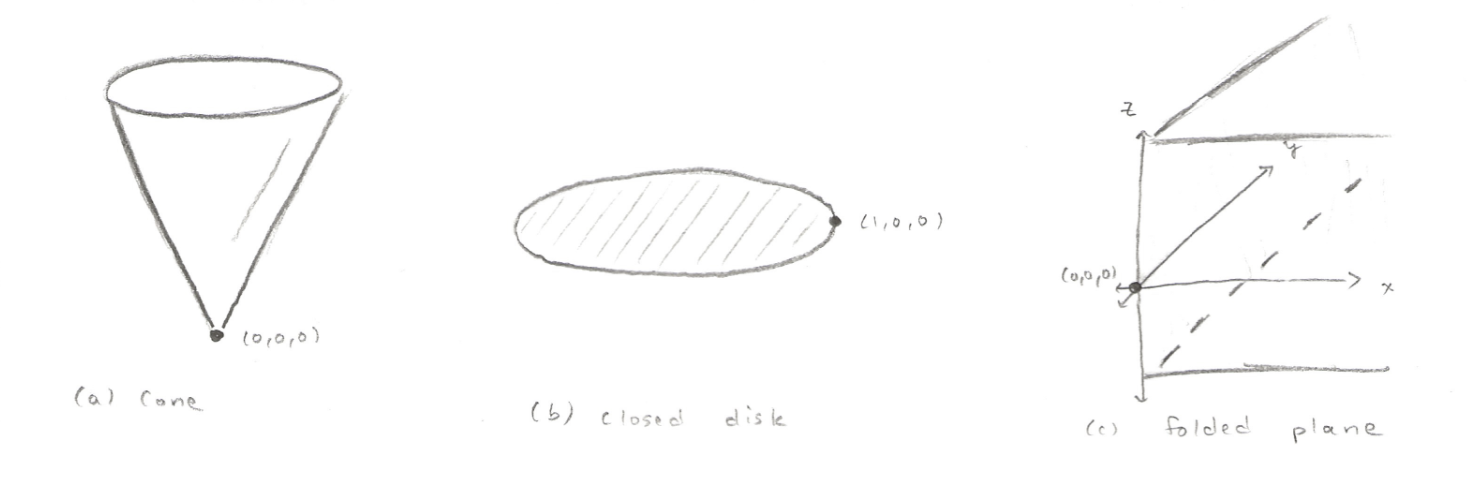
\includegraphics[scale=0.4]{fig/4.1.png}
\end{figure}

\begin{enumerate}
	\item The point $(0,0,0)$ on the cone is not contained in a proper patch since the cone is not differentiable at that point.
	\item Any point along the boundary of the closed disk, for example $(1,0,0)$, is not contained in a proper patch, as the derivative does not exist in all directions at these points.
	\item We again take a boundary point, for example $(0,0,0)$, as the derivative is not defined in all directions at this point.
\end{enumerate}

\begin{exer}[]
\S 4.1: \#6.
\end{exer}
The intersection of the monkey saddle with the $xy$-plane is given by
\[
	y^3-3yx^2= y(y^2-3x^2) = 0.
\] This is true when either $y=0$ or $y^2 = 3x^2$, so the intersection is composed of the lines
\begin{align*}
	y &= 0, \\
	y &= \pm \sqrt{3}x. 
\end{align*}
Assuming we take some point $(x,y)$ that does not lie in the intersection of the monkey saddle with the $xy$-plane, $f(x,y)$ will be positive when $y$ and $y^2-3x^2$ both have the same signs, and $f(x,y)$ will be negative when $y$ and $y^2-3x^2$ have different signs.

\begin{exer}[]
\S 4.1: \#9.
\end{exer}
To show that $\mathbf{x}$ is a proper patch, we must show that it is one-to-one, regular, and has a continuous inverse.
\begin{itemize}
	\item \textbf{One-to-one:} If $\mathbf{x}(u,v) = \mathbf{x}(a,b)$, then we have the system
		\begin{align*}
			u+v&=a+b \\
			u-v&=a-b \\
			uv&=ab.
		\end{align*}
		Solving this system yields $u=a$ and $v=b$, so $\mathbf{s}$ is one-to-one.
	\item \textbf{Regular:} The Jacobian of $\mathbf{x}$ is
		\[
		\begin{pmatrix}
			1&1&v \\
			1&-1&u
		\end{pmatrix},
		\] 
		which reduces to
		\[
		\begin{pmatrix}
			1 & 0 & (u+v)/2 \\
			0&1&(v-u)/2
		\end{pmatrix}.
		\] 
		Thus the Jacobian is full rank, which implies that $\mathbf{x}$ is regular.
	\item \textbf{Continuous Inverse:} We can solve for $u$ and $v$ in the system
		\begin{align*}
			x&=u+v \\
			y&=u-v\\
			z&=uv
		\end{align*}
		to show that the inverse of $\mathbf{x}$ is
		\[
			\mathbf{x}^{-1}(x,y,z) = \left( \frac{x+y}{2} ,\frac{x-y}{2}  \right).
		\] 
		This is clearly continuous, so $\mathbf{x}$ is proper.
\end{itemize}

Finally, since $z=uv$, we can use our expressions for $u(x,y)$ and $v(x,y)$ calculated just above to get
\[
	z = u(x,y) \; v(x,y) = \left(\frac{x+y}{2}  \right)\left( \frac{x-y}{2}  \right) = \frac{x^2-y^2}{4} ,
\] so the image of $\mathbf{x}$ is the desired surface.

\begin{exer}[]
\S 4.3: \#1.
\end{exer}
For a sphere with radius $r$, we know
\[
	\mathbf{x}(u,v) = (r \cos v \cos u, r\cos v \sin u, r \sin v).
\] We then have:
\begin{enumerate}
	\item
		\begin{align*}
			f(\mathbf{x}(u,v)) &= r^2 \cos^2v\cos^2u + r^2\cos^2v\sin^2u \\
					   &= r^2\cos^2v.
		\end{align*}

	\item 
		\begin{align*}
			f(\mathbf{x}(u,v)) &= \left[ r\cos v(\cos u-\sin u) \right]^2 + r^2 \sin^2 v \\
					   &= r^2\cos^2v\left[ \cos^2u-2\cos u\sin u+\sin^2u \right]+r^2\sin^2v \\
					   &= r^2\cos^2v\left[ 1-2\cos u \sin u \right]+r^2\sin^2v \\
					   &= [r^2\cos^2v + r^2 \sin^2v] - 2r^2 \cos^2v \cos u\sin u \\
					   &= r^2(1- 2\cos^2v \cos u \sin u).
		\end{align*}
\end{enumerate}

\begin{exer}[]
\S 4.3: \#6.
\end{exer}
\begin{enumerate}
	\item 
		\begin{figure}[H]
			\centering
			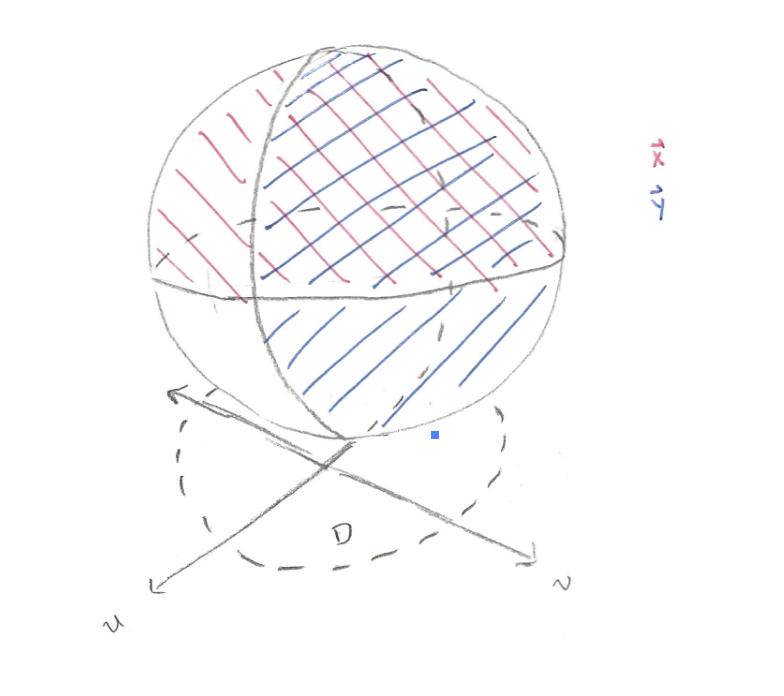
\includegraphics[scale=0.6]{fig/4.3.png}
		\end{figure}
		

		In the next two parts of this problem, we use the fact that the inverses of $\mathbf{x}$ and $\mathbf{y}$ are
		\begin{align*}
			\mathbf{x}^{-1}(p_1,p_2,p_3) &= (p_1,p_2),
			\mathbf{y}^{-1}(p_1,p_2,p_3) &= (p_3,p_1).
		\end{align*}

	\item The function $\mathbf{y}^{-1}\mathbf{x}$ is defined on
		\[
			\left\{ (u,v) \in \mathcal{D} \;|\; \mathbf{x}(u,v) \in \mathbf{y}(\mathcal{D}) \right\} = \left\{ (u,v) \in \mathcal{D} \;|\; v \geq 0 \right\},
		\] and it is given by
		\[
			(\mathbf{y}^{-1}\mathbf{x})(u,v) = \mathbf{y}^{-1}(u,v,f(u,v)) = (f(u,v),u).
		\] 

	\item The function $\mathbf{x}^{-1}\mathbf{y}$ is defined on
                \[                        \left\{ (u,v) \in \mathcal{D} \;|\; \mathbf{y}(u,v) \in \mathbf{x}(\mathcal{D}) \right\} = \left\{ (u,v) \in \mathcal{D} \;|\; u \geq 0 \right\},
                \] and it is given by
                \[
                        (\mathbf{x}^{-1}\mathbf{y})(u,v) = \mathbf{x}^{-1}(v,f(u,v),u) = (v,f(u,v)).
                \]
\end{enumerate}

\begin{exer}[]
\S 4.3: \#8.
\end{exer}
\begin{enumerate}
	\item In the proof of Lemma 3.6, we see that any $\alpha'(t)$ can be written
		\[
			\alpha'(t) = \frac{d \alpha_1}{d t} \mathbf{x}_{u} + \frac{d \alpha_2}{d t} \mathbf{x}_{v}.
		\] 
		Then we have
		\[
			\alpha'(t) = \sqrt{2} \mathbf{x}_{u}(\alpha(t)) + e^t \mathbf{x}_{v}(\alpha(t).
		\] 

		\item We manually calculate
			\begin{align*}
				\mathbf{x}_{u} &= (-v \sin u, v \cos u, 0) \\
				\mathbf{x}_{v} &= (\cos u, \sin u, 1),
			\end{align*}
			which implies
			\begin{align*}
				{\Vert{\mathbf{x}_{u}}\Vert} &= v = e^t \\
				{\Vert{\mathbf{x}_{v}}\Vert} &= \sqrt{2}.
			\end{align*}

			We now show that $\alpha' \cdot (\mathbf{x}_{u}/{\Vert{\mathbf{x}_{u}}\Vert}) = \alpha' \cdot (\mathbf{x}_{v}/{\Vert{\mathbf{x}_{v}}\Vert})$. Since 
			\[
			\mathbf{x}_{u} \cdot \mathbf{x}_{v} = v\cos u \sin u - v \cos u \sin u = 0,
			\] we have
			\[
			\alpha' \cdot \frac{\mathbf{x}_{u}}{{\Vert{\mathbf{x}_{u}}\Vert}} = \sqrt{2} {\Vert{\mathbf{x}_{u}}\Vert}+ e^t \frac{\mathbf{x}_{u}\cdot \mathbf{x}_{v}}{{\Vert{\mathbf{x}_{u}}\Vert}}  = \sqrt{2} {\Vert{\mathbf{x}_{u}}\Vert} = \sqrt{2} e^t 
			\] and
			\[
			\alpha' \cdot \frac{\mathbf{x}_{v}}{{\Vert{\mathbf{x}_{v}}\Vert}} = e^t {\Vert{\mathbf{x}_{v}}\Vert} = \sqrt{2} e^t.
			\] Since they are equal, $\alpha'$ has the same angle with both $\mathbf{v}_{u}$ and $\mathbf{x}_{v}$, i.e. it bisects them.
\newpage
		\item A sketch of the cone and the curve $\alpha$ is below.
			\begin{figure}[H]
				\centering
				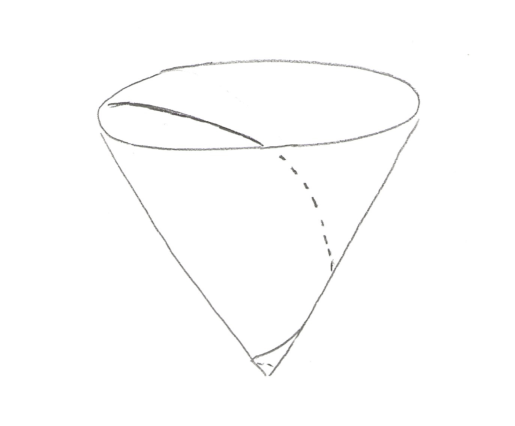
\includegraphics[scale=0.6]{fig/cone.pdf}
			\end{figure}
			
\end{enumerate}

\begin{exer}[]
\S 4.3: \#9.
\end{exer}
\begin{enumerate}
	\item The Euclidean tangent plane is the collection
		\[
			\overline{T}_{\mathbf{p}}(\mathcal{M}) = \left\{ \mathbf{r} \;|\; (\mathbf{r}-\mathbf{p})\cdot \mathbf{z}=0 \right\}.
		\] Thus $\mathbf{v}_{\mathbf{p}}$ is a tangent point of $M$ at $\mathbf{p}$, i.e. $\mathbf{v} \cdot \mathbf{z} = 0$, if and only if $(\mathbf{v} + \mathbf{p}-\mathbf{p}) \cdot \mathbf{z}=0$ if and only if $\mathbf{v} + \mathbf{p} \in \overline{T}_{\mathbf{p}}(\mathcal{M})$.

	\item Every tangent vector at $\mathbf{x}(u,v)$ is a linear combination of $\mathbf{x}_{u}$ and $\mathbf{x}_{v}$, so $\overline{T}_{x(u,v)}(\mathcal{M})$ is spanned by $\mathbf{X}_{u}$ and $\mathbf{x}_{v}$. This means that both are orthogonal to $\mathbf{z}$, and since we're operating in only 3 dimensions, we can take their cross product to yield a vector parallel to $\mathbf{z}$. This means
		\[
			(\mathbf{r}-(\mathbf{x}(u,v)) \cdot \mathbf{z}=0 \iff (\mathbf{r}-\mathbf{x}(u,v))\cdot (\mathbf{x}_{u}\times \mathbf{x}_{v}) = 0.
		\] 

	\item $\nabla_{}g$ is normal to $\mathcal{M}$, so $(\nabla_{}g)(\mathbf{p})$ is normal to $\mathcal{M}$ at $\mathbf{p}$, i.e. parallel to $\mathbf{z}$. Thus
		\[
			( \mathbf{r}-\mathbf{p})\cdot \mathbf{z} = 0 \iff (\mathbf{r}-\mathbf{p}) \cdot (\nabla_{}g)(\mathbf{p}) = 0.
		\] 
\end{enumerate}

\begin{exer}[]
\S 4.4: \#2.
\end{exer}
\begin{enumerate}
	\item For property (1), suppose $\mathbf{v}$ is tangent to $\mathbf{p}$, then
		\begin{align*}
			(f_1\;du_1+f_2\;du_2)(\mathbf{v}) &= \phi(U_1(\mathbf{p}))du_1(\mathbf{v}) + \phi(U_2(\mathbf{p}))du_2(\mathbf{v}) \\
							  &= \phi(U_1(\mathbf{p})v_1+U_2(\mathbf{p})v_2) \\
							  &= \phi(\mathbf{v}).
		\end{align*}
		For property (2), suppose $\mathbf{w}$ is also tangent to $\mathbf{p}$, then
		\begin{align*}
			(g\;du_1 \;du_2)(\mathbf{v},\mathbf{w}) &= \eta(U_1(\mathbf{p}),U_2(\mathbf{p})) (v_1w_2-w_1v_2) \\
								&= \eta(U_1(\mathbf{p}),U_2(\mathbf{p})) (v_1w_2-v_2w_1).
								\intertext{Then by Lemma 4.2, this becomes}
								&= \eta(v_1U_1(\mathbf{p})+v_2U_2(\mathbf{p}), w_1U_1(\mathbf{p})+w_2U_2(\mathbf{p})) \\
								&= \eta(\mathbf{v},\mathbf{w}).
		\end{align*}

	\item For property (3), we have
		\begin{align*}
			\phi\wedge \psi &= (f_1\;du_1+f_2\;du_2)\wedge(g_1\;du_1+g_2\;du_2) \\
					&= f_1g_1 \;du_1\; du_1 + f_1g_2 \;du_1\; du_2 + f_2g_1 \;du_2\; du_1 + f_2g_2 \;du_2\; du_2 \\
					&= (f_1g_2-f_2g_1)du_1\;du_2.
		\end{align*}

		For property (4), we have
		\begin{align*}
			df(\mathbf{v}) = \mathbf{v}[f] &= (\sum v_i U_i(\mathbf{p}))[f] \\
						       &= \sum v_i (U_i(\mathbf{p})[f]) \\
						       &= \sum v_i \frac{\partial f}{\partial u_i} (\mathbf{p}) \\
						       &= \sum du_i(\mathbf{v}) \frac{\partial f}{\partial u_i} (\mathbf{p}).
		\end{align*}

		For property (5), we can use property (4) to get
		\begin{align*}
			d\phi &= df_1 \wedge du_1 + df_2 \wedge du_2 \\
			      &= \frac{\partial f_1}{\partial u_1} du_1\;du_1 + \frac{\partial f_1}{\partial u_2} du_2\;du_1 + \frac{\partial f_2}{\partial u_1} du_1\; du_2 + \frac{\partial f_2}{\partial u_2} du_2\;du_2 \\
			      &= \left( \frac{\partial f_2}{\partial u_1} -\frac{\partial f_1}{\partial u_2}  \right)du_1 \;du_2.
		\end{align*}
\end{enumerate}

\begin{exer}[]
\S 4.4: \#4.
\end{exer}
\begin{enumerate}
	\item 
		\begin{align*}
			d(fgh) &= (df)(gh) + f\;d(gh) \\
			       &= gh \; df + f\left[ (dg)h+g\;dh \right] \\
			       &= gh\;df + fh\;dg + fg\;dh.
		\end{align*}

	\item 
		\begin{align*}
			d(\phi f) = d\left( f\phi \right)&= f\;d\phi+df\wedge \phi \\
				  &= f\;d\phi-\phi\wedge df.
		\end{align*}

	\item 
		\begin{align*}
			(df\wedge dg)(\mathbf{v},\mathbf{w}) &= df(\mathbf{v})dg(\mathbf{w}) - df(\mathbf{w})dg(\mathbf{v}) \\
							     &= \mathbf{v}[f] \mathbf{w}[g]-\mathbf{v}[g]\mathbf{w}[f].
		\end{align*}
\end{enumerate}

\begin{exer}[]
\S 4.4: \#7.
\end{exer}
\begin{enumerate}
	\item By definition,
		\[
			(u,v) = \mathbf{x}^{-1}(\mathbf{x}(u,v)) = \left( \tilde{u}(\mathbf{x}(u,v)), \tilde{v}(\mathbf{x}(u,v)) \right).
		\] 

	\item We have
		\[
			d\tilde{u}(\mathbf{x}_{u}) = \mathbf{x}_{u}[\tilde{u}] = \frac{\partial (\tilde{u}(\mathbf{x}))}{\partial u} = \frac{\partial u}{\partial u} =1.
		\] Similarly,
		\begin{align*}
			d\tilde{u}(\mathbf{x}_{v}) &= \frac{\partial u}{\partial v} =0,\\
			d\tilde{v}(\mathbf{x}_{u}) &= \frac{\partial v}{\partial u} =0,\\
			d\tilde{v}(\mathbf{x}_{v}) &= \frac{\partial v}{\partial v} =1.
		\end{align*}

	\item Let $\mathbf{v}$ be a tangent vector of $\mathbf{x}(u,v)$, then it can be written $\mathbf{v} = a\mathbf{x}_{u}+b\mathbf{x}_{v}$ for some $a,b$. Then using linearity and the properties from part (b), we have
		\begin{align*}
			(f\;d\tilde{u}+g\;d\tilde{v})(\mathbf{v}) &= (f\;d\tilde{u}+g\;d\tilde{v})(a\mathbf{x}_{u}+b\mathbf{x}_{v}) \\
								  &= a\phi(\mathbf{x}_{u})+b\phi(\mathbf{x}_{v}) \\
								  &= \phi(a\mathbf{x}_{u}+b\mathbf{x}_{v}) \\
								  &= \phi(\mathbf{v}).
		\end{align*}
		Now suppose $\mathbf{w}$ is another tangent vector of $\mathbf{x}(u,v)$ given by $\mathbf{w}=c\mathbf{x}_{u}+d\mathbf{x}_{v}$, then by the definition of the wedge product,
		\begin{align*}
			(h\;d\tilde{u}\;d\tilde{v})(\mathbf{v},\mathbf{w}) &= (h\;d\tilde{u}\;d\tilde{v})(a\mathbf{x}_{u}+b\mathbf{x}_{v}, c\mathbf{x}_{u}+d\mathbf{x}_{v}) \\
									   &= \eta(\mathbf{x}_{u},\mathbf{x}_{v})(ad-bc).
									   \intertext{Then by Lemma 4.2, this becomes}
									   &= \eta(a\mathbf{x}_{u}+b\mathbf{x}_{v}, c\mathbf{x}_{u}+d\mathbf{x}_{v}) \\
									   &= \eta(\mathbf{v},\mathbf{w}).
		\end{align*}

\end{enumerate}

\begin{exer}[]
\S 4.5: \#1.
\end{exer}
By Theorem 3.2, $F:\mathbb{R}^3\to N$ is differentiable. Then $F|M$ is a differentiable function from $M$ to $N$. Since $\mathbf{y}^{-1}(F|M)\mathbf{x}$ is then the composition of differentiable functions, it is itself differentiable, so $F|M$ is a mapping of surfaces.

\begin{exer}[]
\S 4.5: \#2.
\end{exer}
I took "meridian" to mean lines extending from pole to pole over only one half of the sphere, and I took "parallel" to mean lines wrapping around the entire sphere horizontally.

\begin{enumerate}
	\item The meridians are moved 180 degrees around the sphere, and the parallels are reflected over the $xy$-plane.
	\item The meridians are made horizontal, then revolved around the $x$-axis. The parallels rotate around the center of the earth, with motion parallel to the $x$-axis.
	\item The parallels are reflected over the $xy$-plane.
\end{enumerate}



\end{document}
